\chapter{Constrained Optimization}\label{app:constrained-optimization}

The standard method of optimizing a function subject to a constraint is called Lagrangian optimization.
Taking a function of two variables $f(x,y)$ as an example, suppose we want to optimize it subject to a constraint of the form $g(x,y)=c$.
In this approach, we define the ``Lagrangian function'' $\mc{L}$ as
\begin{align}
  \mc{L}(x,y,\la)
\equiv
  f(x,y)
-
  \la(g(x,y)-c)
\end{align}
where the parameter $\la$ is called the Lagrange multiplier.
The constrained optimization problem can be solved solved by optimizing $\mc{L}$ with respect to $x$, $y$, and $\la$.
To see why, consider the stationarity conditions for $\mc{L}$.
\begin{align}
  \pd{\mc{L}}{x}
=
  \pd{f}{x}
-
  \la\pd{g}{x}
\overset{!}=0
&&
  \pd{\mc{L}}{y}
=
  \pd{f}{y}
-
  \la\pd{g}{y}
\overset{!}=0
&&
  \pd{\mc{L}}{\la}
=
  c
-
  g(x,y)
\overset{!}=0
\end{align}
The last equation is simply the requirement that the constraint $g(x,y)=c$ be satisfied -- i.e.\ that the point $(x,y)$ lies along the contour of $g(x,y)$ specified by $g(x,y)=c$.
The first two equations correspond to the requirement that the gradients of the function $f(x,y)$ and the constraint surface $g(x,y)$ be parallel
\begin{align}
  \nabla f
=
  \la\nabla g
\end{align}
which is always true at the point $(x,y)$ of closest approach along the line $g(x,y)=c$ to a minimum or maximum of the function $f(x,y)$.
This is best understood visually.
\begin{center}
  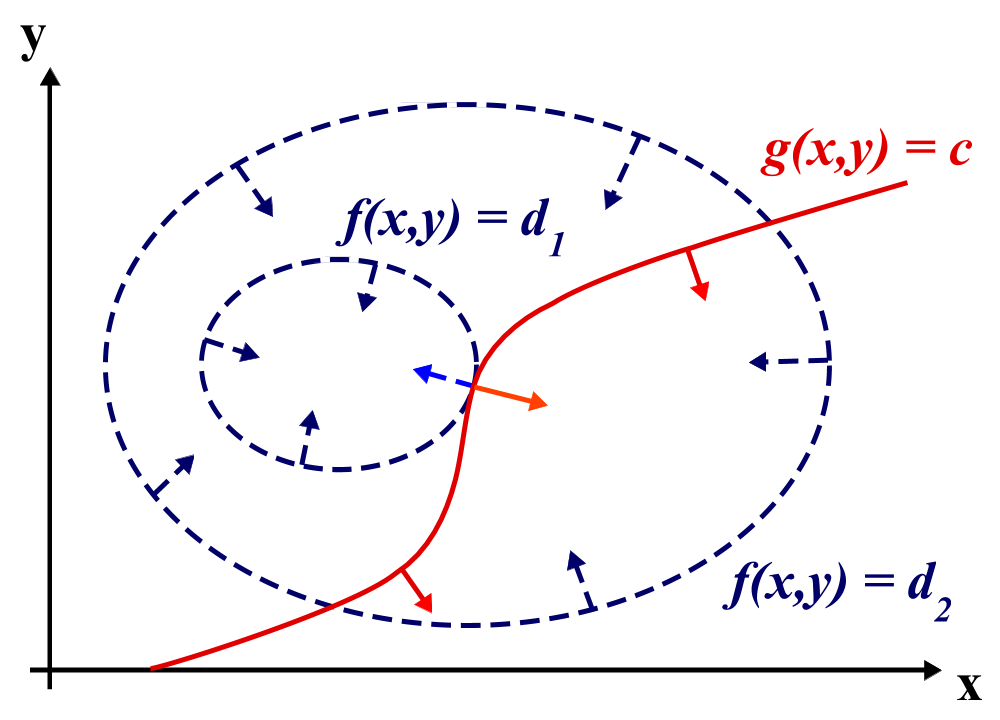
\includegraphics[width=0.5\linewidth]{lagrangian-optimization}
\end{center}
If the gradients were not parallel, we could move along $g(x,y)=c$ to a higher contour of $f(x,y)$ by following the component of $\nabla f$ parallel to $g(x,y)=c$.
